% 2013 湖南卷理科第 19 题：直棱柱 ABCD-A1B1C1D1（TikZ 矢量重绘）。
% 底面 AD=3，BC=1，AB=sqrt3；侧棱 AA1=3。
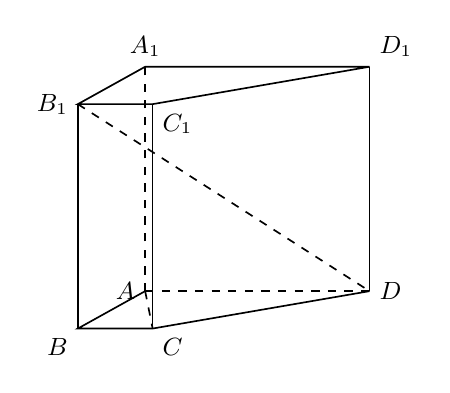
\begin{tikzpicture}[scale=0.95, font=\small, line width=0.6pt]
  \coordinate (A)  at (0,0);
  \coordinate (D)  at (3,0);
  \coordinate (B)  at (-0.9,-0.5);
  \coordinate (C)  at (0.1,-0.5);
  \coordinate (A1) at (0,3);
  \coordinate (D1) at (3,3);
  \coordinate (B1) at (-0.9,2.5);
  \coordinate (C1) at (0.1,2.5);

  % 可见棱
  \draw (A) -- (B) -- (C) -- (D);
  \draw (A1) -- (B1) -- (C1) -- (D1) -- cycle;
  \draw (B) -- (B1);
  \draw (C) -- (C1);
  \draw (D) -- (D1);

  % 不可见棱
  \draw[dashed] (A) -- (A1);
  \draw[dashed] (A) -- (D);
  \draw[dashed] (A) -- (C);
  \draw[dashed] (B1) -- (D);

  \node[left] at (A) {$A$};
  \node[right] at (D) {$D$};
  \node[below left] at (B) {$B$};
  \node[below right] at (C) {$C$};
  \node[above] at (A1) {$A_1$};
  \node[above right] at (D1) {$D_1$};
  \node[left] at (B1) {$B_1$};
  \node[below right] at (C1) {$C_1$};
\end{tikzpicture}
